\newpage
\section{Question 6}
	\subsection{Inverse Kinematics}
	\subsubsection{Theoretical Method}

	
		\subsubsection{Results}

	\subsubsection{Code Listing}
		See Appendix A [9.5]
		
	\subsection{Simulation}

	\begin{figure}[position = here]
		\begin{centering}
			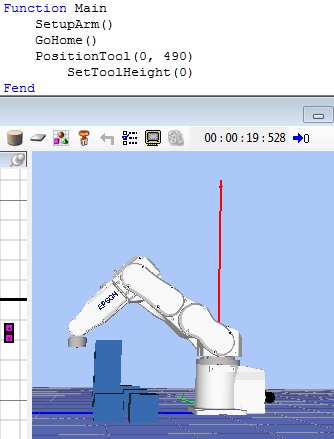
\includegraphics[scale=0.5]{Q6b_a_sim}\\
			\caption [SIMA1]{Simulator Point A}
		\end{centering}
	\end{figure}

	\begin{figure}[position = here]
		\begin{centering}
			\includegraphics[scale=0.5]{Q6b_a_Angles}\\
			\caption [SIMA1]{Simulator Point A Angles}
		\end{centering}
	\end{figure}

	\begin{figure}[position = here]
		\begin{centering}
			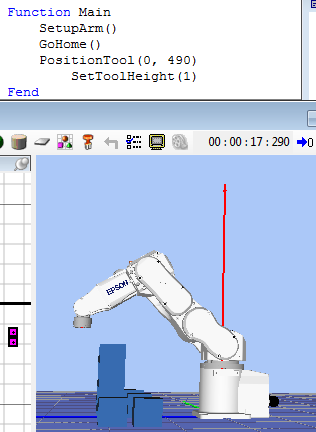
\includegraphics[scale=0.5]{Q6b_b_sim}\\
			\caption [SIMB1]{Simulator Point B}
		\end{centering}
	\end{figure}

	\begin{figure}[position = here]
		\begin{centering}
			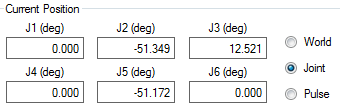
\includegraphics[scale=0.5]{Q6b_b_angles}\\
			\caption [SIMB2]{Simulator Point B Angles}
		\end{centering}
	\end{figure}
\pagebreak